% Packaging
\section{Packaging}
\subsection{Test your application}
\begin{frame}[fragile]{Test your application}
    \begin{block}{Development}
        Run tests while developing using pytest.
        \begin{minted}{bash}
python build.py pytest
        \end{minted}
    \end{block}
    \pause
    \begin{block}{Multi-environment}
        Once development is done, run tests against all different interpreters supported to check compatibility.
        \begin{minted}{bash}
python build.py tox
        \end{minted}
    \end{block}
    \pause
    \begin{block}{Continuous Integration}
        Development is done, tests pass in every environment, so code can be uploaded to repository safely. Once a commit is done:
        \begin{description}
            \item[Travis] run tests in every environment and will notify in case any test didn't pass. When all tests pass,
            \item[Codecov] records current code coverage. In the same commit,
            \item[ReadTheDocs] gets the code, build docs and updates the project's doc page.
        \end{description}
    \end{block}
    \note {
        Testeamos en tres fases diferentes, con objetivos diferentes:
        \begin{enumerate}
            \item Development para comprobar que el código es correcto conforme a los tests.
            \item Multi-environment para comprobar que el código es correcto en diferentes intérpretes de python.
            \item CI para comprobar que la calidad del código y los tests no disminuye con nuevas versiones.
        \end{enumerate}
    }
\end{frame}

\subsection{Creating a package}
\begin{frame}[fragile]{Package types}
    \begin{block}{Egg}
        Source distribution.
        \begin{minted}{bash}
python setup.py sdist
        \end{minted}
    \end{block}
    \pause
    \begin{block}{Wheel}
        Built and binary distribution.
        \begin{minted}{bash}
python setup.py bdist_wheel
        \end{minted}
    \end{block}
    \note{
        Hay dos tipos de paquetes en Python: \emph{egg} y \emph{wheel}. 
        
        Los primeros, \emph{source distribution}, necesitan construirse al instalarlos. Los segundos, \emph{built or binary distribution}, simplemente necesitan ser movidos al directorio correcto. 
        
        Para entender la diferencia entre unos y otros, en cuanto a tiempo de instalación, podemos tomar como ejemplo \emph{numpy}, \emph{scipy} and \emph{pandas}.
    }
\end{frame}

\begin{frame}{Builder}
    \begin{figure}
        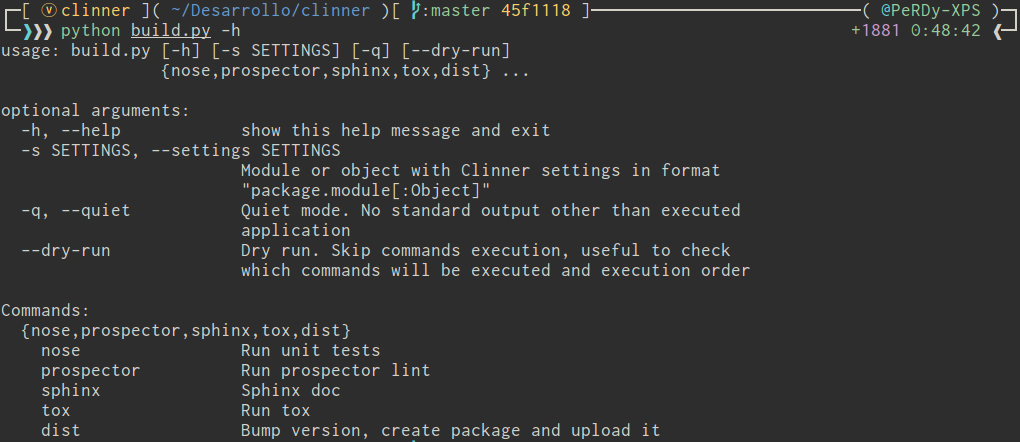
\includegraphics[width=\textwidth,height=0.8\textheight,keepaspectratio]{build_help.png}
    \end{figure}
    \note {
        Aquí se pueden ver las utilidades dentro del script \texttt{build.py}, entre las que encontramos comandos para:
        \begin{itemize}
            \item Generar la documentación.
            \item Realizar el análisis estático de código. 
            \item Lanzar los tests con pytest o con tox. 
            \item Empaquetar y distribuir la applicación.
        \end{itemize}
    }
\end{frame}

